\clearpage
\section{Supplemental Information}
\label{sec:supplement}
\renewcommand{\thefigure}{S\arabic{figure}}
\setcounter{figure}{0}

Figure \ref{sfig:orth} demonstrates that orthogonality tends to increase as we add connections of equal order of magnitude to a graph.  The figure was generated by first creating an all-to-all connected graph having 16 nodes.  Rate constants were chosen randomly from the distribution $Exp[\mathcal{N}(0,\frac{1}{3})]$.  For each of the $c = \text{`connectivity fractions'}$ in Figure \ref{sfig:orth}, a random set of $1 - c*(16^2-16)/2$ connections was then chosen for deletion and removed bidirectionally.  These random deletion sets were chosen 1000 times for each connectivity fraction considered.  The mean and standard deviation of these 1000 samples is plotted.  Graph sparsity 0 corresponds to a $16\times16$ grid graph.

%shows the average orthogonality for graphs with 16 nodes.  First, a random all to all connected graph was created with rate constants chosen randomly from the distribution $Exp[\mathcal{N}(0,\frac{1}{3})]$. Then a random set of connections is generated corresponding to the connectivity fraction of the total $(16^2-16)/2$ links and these connections are removed symmetrically.  Connections to delete are randomly chosen 1000 times for each sparsity and the distribution of the orthogonality for the subgraph between nodes 1 and 16 is computed.  The mean and standard deviation of this distribution is plotted.
\begin{figure}[htpb]
\resizebox{0.95\columnwidth}{!}{
\pgfplotsset{yticklabel style={text width=5em,align=right}}

\resizebox{0.4\columnwidth}{!}{
\subfigure{
% This file was created by matlab2tikz.
%
%The latest updates can be retrieved from
%  http://www.mathworks.com/matlabcentral/fileexchange/22022-matlab2tikz-matlab2tikz
%where you can also make suggestions and rate matlab2tikz.
%
\definecolor{mycolor1}{rgb}{0.00000,0.44700,0.74100}%
%
\begin{tikzpicture}
%\node[] at (-2,7) {\huge (b)};

\begin{axis}[%
%width=4in,
%height=4in,
%at={(0in,0in)},
scale only axis,
xmin=0,
xmax=1,
xtick={0, 0.2, 0.4, 0.6, 0.8, 1},
xlabel style={font=\Large\bfseries\color{white!15!black}},
xlabel={Connectivity, 0=Grid},
ymin=-2.5,
ymax=0.5,
yticklabel style = {font=\Large},
ylabel style={font=\huge\bfseries\color{white!15!black}, at={(axis description cs:-0.15,0.5)}},
scale ticks below exponent=2,
ylabel={$\Theta$},
axis background/.style={fill=white},
legend style={legend cell align=left, align=left, draw=white!15!black}
]
\addplot [color=mycolor1, line width=2.0pt, draw=none, mark=square, mark options={solid, mycolor1}]
 plot [error bars/.cd, y dir = both, y explicit]
 table[row sep=crcr, y error plus index=2, y error minus index=3]{%
1	0.0158897932895343	0.0219638609519872	0.0219638609519872\\
0	-2.19152922410445	0.0442727133533317	0.0442727133533317\\
0.1	-1.26900238075602	0.113140127221996	0.113140127221996\\
0.2	-1.13717407560137	0.105399483670646	0.105399483670646\\
0.3	-1.00117652331271	0.088778703694582	0.088778703694582\\
0.4	-0.860142584690047	0.0752706537627627	0.0752706537627627\\
0.5	-0.726084325807173	0.0648688752958107	0.0648688752958107\\
0.6	-0.588945001891375	0.0557394993663173	0.0557394993663173\\
0.7	-0.444804928347819	0.0432954017554721	0.0432954017554721\\
0.8	-0.287006316742788	0.0332660232213172	0.0332660232213172\\
0.9	-0.132989953746229	0.0271438744901984	0.0271438744901984\\
};

\end{axis}

\end{tikzpicture}%
}
} 
}
\caption{As a graph becomes more connected, orthogonality increases.  Orthogonality is plotted against varying connectivities of a 16 node graph, generated as described in the main text of this section.  Zero connectivity corresponds to a $16\times 16$ grid graph, by convention.}
\label{sfig:orth}
\end{figure}

Figure \ref{sfig:kin_sim} shows the relationship between orthogonality and error for the Ninio-Hopfield model in the kinetic regime $(\gamma=0,\delta=\delta_p=1)$.  High orthogonality and high dissipation are necessary for low error.
\begin{figure}[htpb]
\resizebox{0.95\columnwidth}{!}{
% This file was created by matlab2tikz.
%
%The latest updates can be retrieved from
%  http://www.mathworks.com/matlabcentral/fileexchange/22022-matlab2tikz-matlab2tikz
%where you can also make suggestions and rate matlab2tikz.
%
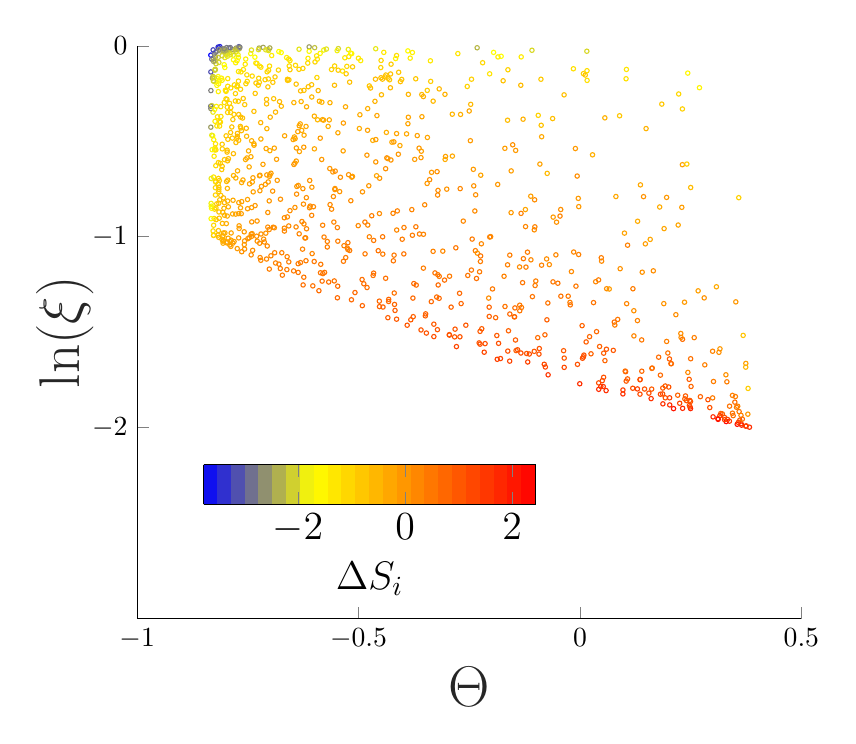
\begin{tikzpicture}

\begin{axis}[%
scale only axis,
xmin=-1,
xmax=0.5,
xtick={-1,-0.5, 0, 0.5},
xlabel style={font=\huge\bfseries\color{white!15!black}},
xlabel={$\Theta$},
ymin=-3,
ymax=0,
ytick={0,-1,-2},
ylabel style={font=\huge\bfseries\color{white!15!black}, at={(axis description cs:-0.05,0.5)}},
ylabel={$\ln(\xi)$},
axis background/.style={fill=white},
axis x line*=bottom,
axis y line*=left,
legend style={legend cell align=left, align=left, draw=white!15!black}
colormap name=mymap,
colorbar sampled,
colorbar horizontal,
colorbar style={xlabel=$\Delta S_i$,
width=0.5*
\pgfkeysvalueof{/pgfplots/parent axis width},
at={(0.1,0.2)},anchor=south west,
font=\Large,
}
]
\addplot[scatter, only marks, mark=o, mark size=0.7906pt, scatter src=explicit, scatter/use mapped color={mark options={}, draw=mapped color}] table[row sep=crcr, meta=color]{%
x	y	color\\
-0.815615823959797	-0.751791896281566	-0.786206554212047\\
-0.353691213391123	-0.265793202087476	-0.415471450363833\\
0.145856531298344	-1.79741473363579	1.08187343936985\\
-0.177977103344908	-0.054791634422772	-1.69938419315672\\
-0.534853750313016	-0.550374617107488	-0.211642420493991\\
-0.812072689011563	-0.399601823669643	-1.06906005464695\\
-0.823317630070181	-0.74324904010812	-1.05355903473029\\
-0.00383194379160456	-0.798975035377094	-0.0680467386197532\\
-0.806263781587902	-1.02310050087202	-0.38068419444319\\
-0.346850283526788	-1.50421524567005	1.09176179019891\\
0.0603045266803143	-1.27212354108448	0.125301925231952\\
-0.660837993960462	-0.896138338619665	0.162577304778169\\
-0.829419515090726	-0.470944428810399	-1.65677564429756\\
-0.807549671152939	-0.930249059146022	-0.562822088285484\\
-0.726445366638569	-0.20610574576606	-0.964390177447218\\
0.180038605280998	-0.844171277178971	-0.373808754299229\\
-0.81583428045276	-1.00301505731869	-0.601096061011719\\
-0.82178209222782	-0.910691464401183	-0.844047816450217\\
-0.830052234962944	-0.168801296733278	-2.34232698971876\\
0.231610469850911	-1.53696327001097	0.629473863449612\\
-0.724188357195897	-0.191727701039699	-0.875697094821136\\
-0.58162153263071	-0.386968494113125	-0.343552960162146\\
-0.780382647940425	-0.204609350350659	-1.08015862307043\\
-0.42660481906617	-0.0962403036488911	-0.875471832867204\\
-0.734157511597854	-0.0593198962577055	-1.69475864445509\\
-0.63940727502809	-0.736524236857563	-0.0531718355541591\\
-0.641214673182448	-0.94864541362279	0.198679556498002\\
-0.77484499862017	-0.484910424643485	-0.588214894455858\\
-0.479208089449945	-0.938744328380655	0.19520312232775\\
-0.699491696396937	-0.37370491426617	-0.506096050735605\\
-0.458501682759224	-0.365460925871844	-0.274999724455774\\
-0.741253532012179	-0.922261944307723	0.0013203490905119\\
-0.634001427875923	-0.41859828290064	-0.271519975753587\\
-0.303666458568016	-0.579380690913824	-0.196775342472619\\
-0.36335632873425	-0.53600689948737	-0.0703545173736389\\
-0.547882397378657	-0.951933809728898	0.340565839500389\\
-0.606024593071701	-0.203819346357847	-0.730010607084221\\
-0.704492152165879	-0.0190696015214708	-1.92590874667715\\
-0.128460178114425	-0.384345111701965	-0.439355810657609\\
-0.769853805493069	-0.942809477781677	-0.140377925063435\\
0.359475008371502	-1.91568046386217	0.522792365934315\\
-0.5532663498938	-0.747470521976626	0.0437976668064345\\
-0.520131101119458	-1.0718662483253	0.441015537709008\\
-0.743051680989002	-0.580833263032974	-0.364489308746227\\
-0.722653941532795	-0.677903460318987	-0.254942446717799\\
-0.586810199705257	-0.0397634690495619	-1.5758817234613\\
0.23683469350999	-1.84894922012286	0.840281616522671\\
-0.781508748832266	-0.359102191279328	-0.825215445353747\\
-0.708825497507374	-0.538097809395571	-0.279058941994461\\
-0.278926157674583	-1.57519446392014	1.28611933843724\\
-0.0617333428361251	-0.380958663291514	-0.663478553519151\\
-0.697937699709011	-1.09970214634725	0.251191094068572\\
-0.806684814237561	-0.872279555088008	-0.554426643794009\\
-0.594780859888407	-0.0526922739940982	-1.33915957723416\\
-0.554853686242317	-1.23142872782227	0.557197783354534\\
0.300568480799508	-1.94318020499565	1.76446146057585\\
0.353477635311851	-1.89294156208446	0.453238456472659\\
-0.53295023284201	-1.04682432817084	0.343252294115541\\
-0.743542860978541	-0.0407649253951749	-1.73263119601578\\
-0.225623955012265	-1.56244349636643	1.12281089481341\\
0.129832001540029	-1.43905969156304	0.289554496807595\\
-0.816001157273586	-0.010043019577085	-3.26145429424616\\
-0.722856266467171	-0.758953847187861	-0.100278986909286\\
0.248575386094584	-1.89135568381677	1.4143138729181\\
-0.742624198042372	-1.09508847815579	0.144189856304151\\
-0.0148396130003385	-0.12020194614618	-1.19570641417481\\
-0.813140973166755	-0.00437199116308036	-3.4885588179505\\
0.0775033604602725	-1.4469534154687	0.664164352107472\\
-0.78243357108914	-0.679397864055594	-0.507443433920045\\
0.135578140442364	-1.82419125710221	1.17801073446263\\
-0.600212716846762	-1.12954710447568	0.481496461433941\\
-0.567495712481718	-1.23699945049881	0.580426282693952\\
0.321654128812483	-1.92803166320307	0.818696120454435\\
-0.58233097672791	-1.23219388456293	0.604900447229966\\
-0.80084021359983	-0.232327856477006	-1.24807318821205\\
-0.132703981659564	-0.0579920635223283	-1.38592055588697\\
-0.22563986671789	-1.49551253811692	0.954065305792851\\
-0.756043633524512	-0.0964568416180298	-1.31948266740265\\
-0.522556485259594	-0.674970079621221	0.0338072267725698\\
0.044366784834641	-1.57470244826723	0.829758644388151\\
-0.110706872657844	-1.12080196157059	0.223560260412818\\
-0.33513780872737	-0.662610023308604	-0.0829040591852886\\
0.00772281393527408	-0.145708000818994	-0.918507696711938\\
-0.16350744658619	-1.1469710061601	0.339929904641019\\
0.0158881921279249	-0.130325074788261	-1.17543852160907\\
-0.623706913130579	-1.2118674078983	0.498570457485676\\
0.177744509503947	-1.63065380774016	0.682455107204125\\
-0.797827735384003	-0.00926542806724253	-2.80351350087885\\
-0.547097123931936	-1.25889753103685	0.631396640185171\\
-0.733764631527641	-0.836633450892284	-0.045157769772607\\
-0.662506018504248	-0.0614373039018803	-1.43311304809362\\
-0.275776496245414	-0.0408397196997476	-1.30087041833516\\
-0.107445581772625	-1.31356769875679	0.53568107312034\\
-0.700353935278479	-0.549262698138716	-0.386114676834256\\
-0.350634474632121	-0.832626816726356	0.211924178485134\\
-0.323580617428282	-1.31566447543468	0.650501471954776\\
-0.57799050637001	-1.00150157505083	0.332639673732065\\
-0.773772489900716	-0.0185961411149292	-2.25546613098716\\
-0.722409611937061	-1.10900191203018	0.216756290993977\\
-0.598389777863771	-0.0845587233032599	-1.03540087212686\\
-0.689508942986178	-1.0836552049374	0.292734904017061\\
-0.585430427468183	-1.14433857487938	0.45323619793125\\
-0.0450427662986914	-0.891653363727011	0.303971507316679\\
-0.422209129874237	-0.877131631219605	0.285331154373372\\
-0.681003098656998	-0.126903768824193	-1.00408454589842\\
-0.437206058654507	-0.45355893940109	-0.39766397919439\\
-0.783124340981706	-0.0488647542029979	-1.93260503808817\\
-0.833580543142595	-0.136939233532645	-3.13320917406572\\
-0.623326853904739	-0.233348103260341	-0.739471229953357\\
-0.00902128437781258	-1.25862679872458	0.467476524947571\\
-0.824216791146621	-0.395434184322077	-1.41171876905941\\
-0.806534143325005	-0.0242449127886784	-2.46170695137632\\
-0.588521530241238	-0.290383100099856	-0.457918275348835\\
-0.337119327870091	-0.18638344429259	-0.890789254604274\\
-0.824936105268584	-0.545382946417721	-1.31087768840303\\
-0.823272965983909	-0.709262866441175	-1.093955148123\\
-0.690193005197009	-0.952831132121466	0.0910852938245944\\
-0.0806410996236866	-1.66785891970597	1.20310579466955\\
-0.0434602084186018	-0.857384966846449	0.098048929822254\\
-0.760473460837838	-0.275986779159049	-0.759649008056135\\
-0.269703027378322	-0.359496348507047	-0.412677123911569\\
-0.515475533632127	-0.0405582232381783	-1.48422592084729\\
-0.171471504510937	-1.2069554896374	0.317894129705854\\
-0.770180820470196	-0.00439164160780345	-3.00553501700784\\
-0.417690623119379	-1.38594337748013	0.885121054261791\\
-0.822243530505892	-0.545182185853895	-1.18289274007817\\
-0.769357607965275	-0.0154637939311217	-2.3362203192248\\
-0.714408717037977	-1.01261977405381	0.0795501484502908\\
-0.788625180406414	-0.220430653399282	-1.11551126083134\\
-0.433823965152048	-1.42393215837415	0.927621790603275\\
-0.322719881733018	-0.659200493524618	0.100508974910604\\
-0.221809436335176	-1.48167331766636	0.916123850604952\\
-0.449433091830009	-0.167247102693201	-0.595836791327825\\
0.379189055714994	-1.92897437114968	-0.059510146331925\\
-0.438369303816996	-0.153037206178149	-0.782479644100621\\
-0.614208596332641	-0.0657938110149402	-1.41360936670408\\
-0.0753380788600035	-1.1162558661308	0.123101911669376\\
-0.619541211320687	-1.00562459036031	0.189116390975354\\
-0.777248082560873	-0.692221617917253	-0.459763478078609\\
-0.679812964786896	-1.14326924960411	0.358100576928417\\
-0.828922647236075	-0.160693304096567	-2.18706987726078\\
-0.640985741499268	-0.200680026842741	-0.725853198529947\\
-0.796500815587047	-0.0435644630944353	-1.99337767787597\\
-0.643757074969433	-0.614388658798311	-0.125395383482026\\
-0.803371492306912	-0.297008188166552	-1.16951134470545\\
-0.317882952236499	-0.225654209353703	-0.555975071287847\\
-0.820367027132936	-0.827832820237345	-0.862907369197615\\
-0.452398371173867	-0.693644853785061	-0.00189821074870469\\
-0.710413426978224	-0.725592682463908	-0.11798901889625\\
-0.370920162041577	-0.172756073233246	-0.787832306736948\\
-0.123244768406764	-0.857453804067225	-0.259848703018206\\
-0.578633959273803	-0.0221373878752133	-1.83756507667459\\
-0.305855250018616	-1.22680326629256	0.653952587023636\\
-0.634445084947108	-0.0179321766101319	-1.90674238385676\\
0.346016272124015	-1.93676776658374	0.661271438588738\\
0.0155220048535217	-0.0284236866087961	-2.0178046816458\\
-0.70778649095597	-0.30415020044736	-0.636455978457824\\
-0.282074827389965	-1.48386068829103	1.0147379067439\\
-0.132051478994889	-1.37017293660425	0.438988116613552\\
-0.358963381766017	-1.48813059387999	1.01862456317335\\
-0.0355752695541633	-1.63530363205532	0.951074531022663\\
-0.572678854342426	-0.0169691612872633	-1.9343530404214\\
-0.0265788358821584	-1.31127068672497	0.47442929483051\\
0.368565132006306	-1.51664530412869	-0.748617839041625\\
-0.640759086703992	-0.603592074622351	-0.173628731330265\\
-0.339492144380444	-0.7010214155435	0.111189306803487\\
-0.690325530361418	-0.535793253099448	-0.245178070208493\\
-0.618636238955178	-0.422385515072629	-0.330023274579439\\
-0.556867892868995	-0.789358790538408	0.128171412345169\\
0.331767966804967	-1.75956792688987	0.390305378017145\\
-0.782659045318893	-0.5648346634279	-0.601306215709615\\
0.158655670998188	-1.01387878044427	-0.268389150772325\\
-0.594019335581112	-0.16612765878314	-1.07342778329713\\
-0.377285628256839	-1.32108573468236	0.722774586649351\\
-0.731710338579631	-0.195104984758855	-0.859519229599732\\
-0.82626875173508	-0.578347004160909	-1.34121952920319\\
-0.667040179317935	-0.47126158324253	-0.26230681456689\\
-0.806079645387252	-1.03349320886839	-0.369870846310643\\
-0.335746042381284	-1.33975659670445	0.738661005811036\\
0.250855345445409	-1.78409678547009	0.765414237572921\\
-0.599748300643108	-0.539580388464565	-0.296824675636832\\
-0.379782033226106	-0.857907041950972	0.269158881778216\\
-0.362383166655342	-0.98554081945812	0.37315877065094\\
-0.586550028332358	-0.48354721469004	-0.116446656306444\\
-0.692651123759493	-0.949929717092705	0.162978139364782\\
-0.516073612703967	-1.32995694384273	0.736197765428753\\
0.0374607421488466	-1.49695805947349	0.735385256277613\\
-0.657690735119129	-0.943459932183975	0.1662530972279\\
-0.674486023841057	-0.316347956108047	-0.56952867352832\\
0.0598038069654021	-1.58894108183443	1.00090047513401\\
-0.740414063187212	-0.983772074660838	0.018553560195273\\
-0.827443032170591	-0.992264102633094	-0.982510105413489\\
-0.802712188291976	-0.887354508655696	-0.477642785408967\\
-0.41251852261145	-0.8646475659816	0.318714692327658\\
0.0119951403041063	-0.153165996443407	-0.7747831775894\\
0.140605678517606	-1.18564206144602	0.0536191542092135\\
-0.21622748053812	-1.60461601673388	1.26571026371994\\
-0.66198368455576	-1.17188110978254	0.403374365095042\\
0.0354381162354974	-1.23552829106602	0.244468822378231\\
-0.747132161757904	-0.634277183121686	-0.337830482306248\\
-0.56457312238105	-0.29793015247581	-0.456777857012734\\
-0.617932897411427	-0.795235426852084	0.0817973585936764\\
-0.436190040844512	-0.587005209102523	0.090832035401903\\
-0.785104803486222	-0.0187061559209944	-2.42972839854061\\
-0.634101191018956	-0.984624169716577	0.267686887209579\\
-0.776327131454754	-0.0118124973756453	-2.47418529950229\\
-0.163561621389002	-0.38970083247339	-0.639064051303048\\
-0.558080009967986	-0.660651347752944	-0.039413333347828\\
-0.095361477446686	-1.52845795140212	0.679391755378611\\
0.104088771159968	-0.172557456538991	-1.20653891689849\\
-0.703264327306974	-0.0247862379337576	-1.95874634920087\\
0.249712511200362	-1.89978061980348	1.83171354227553\\
-0.0917978273984108	-1.58527742235291	1.05668657075936\\
-0.808496570220655	-1.01305088269719	-0.42556884032278\\
-0.515369852911581	-0.687707648259663	0.00204534250788926\\
-0.197541208198233	-1.27339168843515	0.462963260537441\\
-0.789042468662654	-0.454127333318282	-0.78130598151299\\
-0.821265558946695	-0.317433088836557	-1.44166623524017\\
-0.74848075784871	-0.550546574401445	-0.397483469414188\\
0.160694219264153	-1.84748370391272	1.61426910629319\\
0.206432446537561	-1.66473729472084	0.630336671648032\\
-0.0499702842939083	-1.24340038971226	0.509946491162994\\
-0.819507362047613	-0.171415620484391	-1.7114151173509\\
0.195663825187044	-0.79398962969226	-0.0468499106522139\\
-0.479385202749917	-0.328758183382831	-0.424950568691279\\
-0.00273899817676893	-0.84219693187004	-0.0709754641973203\\
0.0139381371702962	-1.55087449799446	0.887194965656065\\
-0.327462848565373	-1.18945323717426	0.526093732396522\\
0.195741100301473	-1.54833767161831	0.358809663008724\\
-0.0529155375595358	-0.923525709753119	0.0557248766715468\\
-0.536252348767812	-0.132207945596974	-1.30505726825534\\
-0.158410009303947	-1.40460143324255	0.74376133460196\\
0.0969814263770069	-1.82306451037536	1.67275896155455\\
-0.611623834223752	-0.00572078458855534	-2.5031022703857\\
-0.788852361475961	-0.349176784802529	-0.90548504116823\\
0.288942223972256	-1.85320713971061	1.12285375668811\\
-0.397433395224218	-0.951679824649486	0.357292913747109\\
-0.475717165682353	-1.00022067456355	0.271192558449105\\
-0.118503325097816	-1.08066372371927	0.417430475872455\\
-0.816403527047434	-0.694472519483665	-0.91130254756827\\
0.19263323480462	-1.78161954149928	0.884497148521612\\
-0.833694647370128	-0.426161076006084	-2.50331652693833\\
-0.014195218996776	-1.079919019313	0.242908665894494\\
-0.250173575961959	-0.341395444051408	-0.298663284274829\\
0.0811747390283365	-0.789294302925924	-0.298372543796361\\
-0.680077898795345	-0.0301920029931785	-1.69539889872562\\
-0.705026339135218	-0.872831066697881	0.031035458038271\\
-0.401401792030478	-1.01298234665165	0.42939402452442\\
-0.0369622859734415	-1.59676130842988	0.947769101340988\\
-0.388670849207152	-0.0267129343832562	-1.63612587139618\\
-0.331676503874532	-1.07640036364057	0.308500774783429\\
-0.554404764610295	-0.206643016588223	-0.653990580200736\\
0.281902268224049	-1.67087186520154	0.347734808074999\\
-0.000478519698441593	-1.7697961048081	1.65414023450906\\
-0.617477730631874	-0.319240032505877	-0.391158981590522\\
-0.127754327103229	-1.11480943015365	0.434007235155371\\
-0.329973920817246	-1.45777706795369	0.958999305311847\\
-0.0781219735275434	-1.68208099868995	1.25606079668031\\
-0.765569756305001	-0.136788587844748	-1.18948823980625\\
-0.783786748270965	-1.03297662787795	-0.151553200968365\\
-0.73923508637615	-1.07104555577667	0.123045388714208\\
-0.740286243887524	-0.158495417571482	-1.07972010476109\\
-0.101295166716318	-1.25524109690561	0.406495774485697\\
-0.815741316421412	-0.763317907844296	-0.820651741822354\\
-0.235584620767656	-0.78024032549272	0.0969053259489568\\
-0.461138078212019	-0.608171125216398	-0.0417370605874556\\
-0.465874678121579	-1.01922099325563	0.465944193626027\\
-0.820693101608693	-0.0290009544527064	-2.6820669431511\\
-0.345217674015296	-0.720852119386072	-0.0445208414905285\\
-0.70179790725707	-0.812330546715615	-0.034484093448065\\
-0.706507276239246	-0.136084805627235	-1.04562186656116\\
-0.657585591266666	-1.13164664948985	0.393611959457074\\
0.0752555037705165	-1.59502082293501	1.0054943346484\\
-0.783526450322189	-0.808889316265475	-0.347827734833352\\
-0.32062270632238	-0.757335177798089	0.150504043728703\\
-0.833628046173311	-0.0488787408013944	-3.76384622481204\\
0.355119174266023	-1.98198149114583	2.23526057633657\\
-0.243462776502082	-1.01222203841213	0.456117240396471\\
-0.736164244162136	-0.520546928954253	-0.381969536258171\\
-0.815573774853502	-0.824262583017203	-0.744779116421447\\
-0.0719462800380621	-1.72305723036879	1.55373004182723\\
0.271937463665737	-1.83756144938801	0.835987809721666\\
-0.812293489406184	-0.6154877811095	-0.87921147611145\\
-0.179508501565259	-1.63784491344749	1.32840732284303\\
-0.61073942309441	-0.848082675060926	0.144859377001075\\
0.269874043984781	-0.219438233388692	-1.5303827289416\\
0.056406387404218	-1.6486273381102	0.790155720966949\\
-0.419453771657676	-1.2946596994992	0.563140661360987\\
-0.0225630040546525	-1.34387539523032	0.36078248624414\\
-0.817210885415865	-0.0064161481590088	-3.37265980631814\\
-0.233681357209531	-1.21845538582765	0.617727610185481\\
-0.162998494584049	-1.59864888435608	1.10714016939416\\
0.00575248638248715	-1.63630469934419	1.13846752090258\\
-0.378466123275081	-0.0350873133248537	-1.50240172189427\\
-0.0358783939142142	-0.25693039404663	-0.672330731578184\\
-0.092546516328857	-1.61441351794048	1.09519488457132\\
-0.826887795088689	-0.186216990195012	-1.91638151710515\\
-0.414202615272097	-0.459554088205268	-0.243023499481993\\
-0.793132455918861	-0.0124640597095462	-2.68145652934508\\
-0.0875784561984232	-0.416169061970751	-0.731371411594932\\
-0.776165413949159	-0.0318188657796854	-2.02254778546347\\
-0.791522260249876	-0.300941633228025	-0.991782513116153\\
-0.723745134131339	-0.680616431341407	-0.153634595887592\\
-0.466018372033599	-1.1902905487078	0.61804444094212\\
-0.452755498755701	-1.36570392634831	0.809771441576698\\
-0.542667662603685	-0.763512800679567	0.0156771098289565\\
0.318029430189389	-1.92577178824542	0.878928527349875\\
-0.721066057131645	-0.402331174640643	-0.482064345422074\\
-0.545785207580624	-0.014815824637078	-2.0431033488302\\
-0.406546652679447	-0.522320202215603	-0.307493524080719\\
-0.498270381453693	-0.433124194110695	-0.36937061174204\\
-0.0355783801837863	-1.68402979619149	1.22626118202254\\
-0.79547298363631	-0.703365381273812	-0.546403939655635\\
-0.47304102795463	-0.220994923819089	-0.61281710884825\\
-0.353462751760565	-0.98707527130975	0.277989029732526\\
-0.825204643347296	-0.855335072539862	-1.04638010326491\\
-0.766636501379329	-0.227611025130168	-0.958370452024507\\
-0.827422862321248	-0.0682360731379193	-2.41969026205359\\
-0.624490913339131	-0.829186043017845	0.090078136894194\\
-0.8242442725839	-0.127508716606434	-2.09397950612319\\
-0.214223989403997	-1.55962828554766	1.12766887838589\\
-0.757475343183628	-1.06447264277168	0.0474221730081449\\
-0.805382223272092	-0.980287847711795	-0.441418315347135\\
-0.520136194823258	-0.190365027908127	-0.696545283449037\\
-0.822520914470334	-0.627817795284401	-1.14814796246089\\
-0.79694734705789	-0.556555229573677	-0.659877700131803\\
-0.824174624628777	-0.535355551055035	-1.26279081167194\\
-0.136362355294676	-1.15821187276601	0.167619087214239\\
-0.453121604981571	-1.33721134899867	0.743586316663848\\
-0.630890856356147	-0.236144014913908	-0.623379244362089\\
-0.564399043343785	-0.831731930943123	0.188777665121691\\
-0.576821578797494	-1.18679176760678	0.506025180142184\\
0.231828988799073	-1.89850794229697	1.75648412450188\\
-0.566162917933827	-0.388070428442978	-0.316268891198331\\
-0.145155484958737	-0.547900315647675	-0.0859901939666222\\
-0.358269759201713	-0.552107604038762	-0.167577257804316\\
-0.808247319645941	-0.180388598775979	-1.41478349584073\\
-0.382051872489021	-1.43481287335725	0.943867719822606\\
0.0217109595975533	-1.52328540866624	0.747258916488096\\
-0.788504216934351	-1.05038020882061	-0.154221541020639\\
-0.467961156500522	-0.495095860151936	-0.392130743488082\\
-0.831453686215221	-0.0701411781805013	-2.94774585870149\\
-0.778929712180471	-0.0211297893024436	-2.23119977299891\\
-0.809471543620717	-0.169638932010825	-1.49149104964741\\
-0.599971585485796	-0.368421981828995	-0.414591411410928\\
0.103114043304299	-1.70666642832066	1.006157881117\\
-0.697832840939158	-0.66737676461429	-0.185544701062885\\
-0.770728513359794	-0.359805961177268	-0.701517235852629\\
-0.185139518849672	-0.0583935047796798	-1.45429316342795\\
-0.448341057882606	-0.256430762559693	-0.577095415945458\\
-0.646143836616393	-0.297434895197013	-0.488899695001969\\
0.121884548312757	-1.51930558817941	0.264126881916818\\
0.299599626878469	-1.84394273650814	0.439513857641035\\
-0.706262844522015	-1.04847942738361	0.209228691592857\\
-0.634580429640956	-0.123066315360487	-0.976825614318679\\
-0.00629758608609921	-0.682044833546891	0.126196261581652\\
0.316216195307413	-1.58691301692543	-0.05478036215696\\
-0.707832465671564	-0.280593436273266	-0.655738783528945\\
-0.491178085042356	-0.764762437876735	-0.00234286697152022\\
-0.766637353522474	-0.848384252545206	-0.259656642458341\\
-0.732045535163216	-0.0905620823330928	-1.39274303645873\\
0.121650294920406	-1.3874588103304	0.0815926448618805\\
-0.741360379435427	-0.846885702852289	-0.0968526008250297\\
-0.815316161023369	-0.870176889540313	-0.705980004891571\\
-0.526513525367911	-0.10776910933868	-1.08834565491695\\
-0.815472287384347	-0.0870659920379975	-2.02679380110087\\
-0.678517094580967	-0.292364413922714	-0.588057312783619\\
-0.647876410052014	-0.490719290937438	-0.212211007480737\\
-0.771364455618808	-0.0610245687523876	-1.61649153679259\\
-0.263535227693433	-0.918020819295883	0.204829394328685\\
-0.824500832913978	-0.0781386060259953	-2.32515377459385\\
-0.524054048022333	-1.0309985343468	0.459538504240126\\
-0.222644839275736	-1.03682728004365	0.204043146608988\\
-0.814605070933888	-0.902883068293914	-0.694962434931425\\
-0.383445244737052	-0.0645566115905956	-1.40442838510557\\
-0.169607121470432	-0.53688259279992	-0.122316611229196\\
-0.810766879470692	-0.370113025863339	-1.18385065648364\\
-0.816519627220251	-0.967977986463827	-0.690291888409776\\
-0.236261314826662	-1.07280432219022	0.394367935713893\\
-0.676795627003151	-1.16628867289904	0.409099010867467\\
-0.449146328554517	-0.076719816451639	-1.05200256856888\\
-0.0790970424163357	-1.51349180614466	0.740358351548149\\
-0.831476342788286	-0.468312464125175	-1.86719317095415\\
0.337878487107415	-1.88727134832564	0.560008902707303\\
-0.639969399432703	-0.776570950608691	0.0966017428879176\\
-0.799399434582382	-0.238531362814134	-1.24552840663557\\
-0.433295353943584	-0.17009976548929	-0.676320064284382\\
-0.359004266858692	-0.585468671133789	-0.0688286431782785\\
-0.617531697934796	-0.958182627114814	0.25842097809634\\
-0.461840916217014	-0.174657069120326	-0.627706819945371\\
-0.356913740536825	-0.371438712143613	-0.274194483871039\\
-0.148147356560586	-1.41953452390895	0.499150750554466\\
-0.570648283438019	-1.05357033404189	0.372427036673042\\
0.236115960071116	-1.34277647662606	-0.0606012734041439\\
-0.158687602330568	-1.65140693709325	1.33377681485442\\
-0.801885350439571	-0.980017873666545	-0.361697382764001\\
-0.774383564554783	-0.0779385828465559	-1.57633017490356\\
-0.738527836313372	-0.691200911678365	-0.214977313849151\\
-0.373210486059248	-0.594739737883294	-0.0895162800755062\\
-0.144376689762434	-1.59595945864713	0.910986935891914\\
0.35626027620702	-1.88757777335627	0.310042463919192\\
-0.625737284131629	-0.747998087839512	0.0473254441360799\\
-0.462977110053367	-0.290785324571426	-0.465487725549489\\
-0.133343903132611	-1.60879198478906	1.17642777554818\\
-0.548416054062408	-0.0252664069839056	-1.80282081469575\\
-0.610338251823958	-0.705346537380661	0.032271216386939\\
-0.776933838693546	-0.506577226553736	-0.605556613442881\\
0.00887863246965237	-1.61987044608962	1.08681546438234\\
-0.799442231022511	-0.278106272589918	-1.07386655342287\\
0.192679126920496	-1.84352837214481	1.05056627036014\\
0.24369176677078	-1.71038218503726	0.217980218324749\\
-0.34488648656166	-0.233474482975496	-0.874413988019553\\
-0.661377380158141	-1.10437308595382	0.329514067025645\\
-0.155323967854351	-0.655155494226543	-0.14311332386226\\
-0.739984348060574	-0.713284814225974	-0.253569321331007\\
-0.604875722241381	-1.08826129771218	0.26375180046346\\
-0.074639423252983	-1.43504126843516	0.854986596009233\\
-0.741499024951836	-0.497376705982711	-0.423291810276112\\
-0.629647078175029	-0.291804650168763	-0.481235616883162\\
-0.703108585442548	-0.128223192970663	-1.04763217612815\\
-0.609411636572714	-0.839480972843835	0.140709667898605\\
-0.444853123800788	-1.36799709779011	0.820831933289982\\
-0.828721261700612	-0.347399775509108	-1.8672345946986\\
-0.0103758303459207	-0.537960463673413	-0.0575036332568204\\
-0.794064000749799	-0.843315245939814	-0.404456218731167\\
-0.151925232425589	-0.518401193780781	0.0821472537423116\\
-0.736292871591788	-0.512917289566326	-0.416286906028691\\
-0.69619011359818	-0.0509538583643941	-1.41114215842232\\
-0.737954544057756	-0.764945488797162	-0.193596661902242\\
-0.808061698729132	-0.515579809643775	-0.862896794874411\\
-0.82412376423082	-0.123461642792868	-2.04997165708575\\
-0.32997145588651	-1.52285337936829	1.13224588014678\\
-0.475748148174238	-0.210082279186305	-0.799334095423911\\
-0.552774784321115	-0.656168199030396	0.115838705244532\\
-0.693596211068506	-0.191247431858818	-0.802128910770044\\
-0.754808753272025	-0.0693388200760559	-1.46538317369944\\
0.363688679517279	-1.93507346513068	0.318722714624364\\
-0.773357694006267	-0.208514836093485	-1.07972562070629\\
-0.605421831552121	-0.740533544071161	-0.0431929675780832\\
-0.387548202356482	-0.254216248276965	-0.519889710631613\\
-0.605875531761924	-0.887908296445401	0.254285453740792\\
-0.455603204585875	-1.07308084956502	0.569284711577961\\
0.36394250291553	-1.97897383473841	1.42426913551706\\
-0.321898943110175	-1.48663089216352	1.01746896348207\\
0.231263640661843	-0.622690195940963	-0.187531151867183\\
-0.554078121126924	-0.105635724548848	-1.02617708591628\\
-0.424649866977104	-0.504760376423269	-0.307118249992294\\
-0.500801012470053	-0.941816303576009	0.198948175674948\\
-0.819907123520636	-0.207161912327516	-1.63251408175461\\
-0.623761298282455	-0.531016780783907	-0.0905173914294646\\
-0.701644058506043	-1.16921377741826	0.380109742356054\\
-0.683685418986683	-0.704571842005619	-0.0831956479947783\\
-0.591260907824386	-0.234440546195075	-0.550087300014492\\
-0.807392932094197	-0.0155563739670936	-2.68782408627286\\
0.351965041594408	-1.34108898001853	-0.0341414872596898\\
-0.625282484159585	-1.25242181640031	0.618948545800606\\
-0.770719962751886	-0.494748531019649	-0.633655694995511\\
-0.555766823536657	-0.92297204459149	0.282085671456723\\
-0.271060113024285	-1.52395152929763	1.03706875806213\\
-0.81698565218474	-0.722776785324888	-0.904290145799563\\
-0.771310683925868	-0.185061687845614	-1.06959053571583\\
0.22998789684617	-0.845910502132218	-0.127618942027704\\
-0.294873184197152	-1.51515962011587	1.01017425948092\\
-0.0865457028874999	-0.476162920015855	-0.304116156408852\\
0.149262986388608	-0.433475947070646	-0.473445141763454\\
-0.833575890209166	-0.328922915484742	-2.58106403996981\\
-0.295116603900023	-1.51283659503747	1.06576891618896\\
0.119231393971621	-1.79340444414932	1.15291077985132\\
-0.741947433179901	-0.0220662015409756	-1.95625412977887\\
-0.688710174491542	-0.163044172186977	-0.878748232149526\\
-0.397777520876678	-1.08990461723888	0.527560025003242\\
-0.712908795221401	-1.02751600811604	0.144229685199009\\
-0.19504538161633	-0.0344628797362706	-1.69773111665479\\
-0.833021760465319	-0.825499180320666	-1.81417451875316\\
-0.831973242720666	-0.850867596380207	-1.6192030566846\\
-0.239861198812824	-0.73352495563306	0.0496619161226436\\
0.139616510666993	-1.70412924036226	0.726107201433271\\
0.243452427376684	-0.142863114574435	-1.58317965670113\\
0.299561445933665	-1.59953096418115	0.290162381619438\\
-0.782566394320767	-0.0732385568626987	-1.67955577623397\\
-0.827407067828624	-0.687220284166806	-1.29199599300188\\
-0.807775115903311	-0.539873221554131	-0.91003748762023\\
-0.13306973699826	-0.877681339607478	0.339167200288077\\
0.0562016210049955	-0.377240884887284	-0.457937701646717\\
-0.320222820068675	-1.25249527884306	0.704549986458361\\
0.184794381628849	-0.305285657041601	-0.78671061849278\\
-0.720585164441414	-0.1119550851836	-1.14105469208747\\
-0.135958147840232	-1.38757452741867	0.51725735163281\\
-0.823250737623992	-0.781531178667624	-0.995611845528342\\
-0.818717279621128	-0.371577203635635	-1.26638563037735\\
-0.74249250012416	-0.986088771352503	-0.00125066673402651\\
-0.402520280773168	-0.17602757957641	-0.761990968813954\\
0.379613453577909	-1.79437627916318	-0.893636977732219\\
-0.654936415029577	-0.0774921303722034	-1.22589998227328\\
-0.720536924834455	-0.488041223147629	-0.397404183148817\\
-0.581101697006458	-0.93961521862318	0.314893495838746\\
-0.77826465139258	-0.288916673131235	-0.934461627611977\\
-0.795436888596271	-0.171848582287597	-1.26788354418319\\
-0.527983934657091	-0.146577284391696	-0.874588038788967\\
-0.751489112951752	-0.186103367804979	-1.06768636891243\\
0.249675159031492	-1.86256754158157	1.04583387586546\\
0.0283676796095997	-0.570853116923789	-0.399032580377505\\
0.202752319702565	-1.88085728161933	1.66597361487612\\
-0.815266977022925	-0.0201206944535044	-2.62135288209955\\
-0.55355735632288	-0.752861469800901	0.00755568212543913\\
-0.823491152061802	-0.124340911762181	-2.0801294673762\\
0.0970828570754371	-1.80254133480025	1.44261193394324\\
-0.816038857970783	-0.198926686683446	-1.51751872108856\\
-0.701783174114761	-0.961972764279035	0.167301020661142\\
-0.593183694917796	-0.0698394504661624	-1.24640649684893\\
-0.750736265308625	-0.804909252449977	-0.228476727902604\\
-0.787776083262328	-0.980183110376109	-0.264931376655665\\
-0.806822268464008	-0.997974135025451	-0.423416445182862\\
-0.764089527983944	-0.716110964757083	-0.339795823611579\\
-0.725533775131317	-0.170053749935119	-1.00668935977821\\
0.382814841307203	-1.99736513783441	1.67967484065494\\
-0.827275147110752	-0.939814426856417	-1.06798678590057\\
0.249988188721781	-1.63877472665745	0.599578718132186\\
-0.786269471484803	-0.425138567958144	-0.762955279736325\\
-0.80493568619435	-1.01977451955923	-0.361630171803884\\
-0.67474046952072	-0.0352595093692694	-1.65000156460853\\
-0.70474262204298	-0.215210139940876	-0.814930207796466\\
-0.565074765972613	-0.64273673446326	-0.023310676862648\\
-0.206107465355275	-1.32116808180228	0.154812152794253\\
-0.288349184219686	-0.358212833545092	-0.516429145323039\\
-0.657737004825227	-0.0691583131265833	-1.25725817412207\\
-0.431944931796156	-1.32793671872583	0.768003097342659\\
0.0907960623204381	-1.16730832907632	0.0681241111904859\\
-0.10318528222195	-0.963727498132787	0.130735798104873\\
-0.770600960790527	-0.878615116162374	-0.215293114848532\\
-0.769711898357269	-0.956436141024362	-0.157416020180484\\
0.221804134010494	-0.938531990860301	-0.270068827531609\\
-0.77220275655545	-0.0466760075511679	-1.80790105414581\\
-0.42689215440921	-0.597987124654332	0.022292621180936\\
-0.766208354223969	-0.373391521002977	-0.69262980778993\\
0.311733752177282	-1.9526380653424	1.75934500833261\\
-0.496970643068227	-0.36112089482027	-0.36840741391302\\
-0.410204680503159	-0.567817367547401	-0.0551049520874406\\
-0.777591530243912	-0.0887018465840838	-1.4523974298935\\
-0.561149704385631	-0.124373321524296	-0.973324113157323\\
-0.657293936937286	-0.178346882960181	-0.843197802296816\\
-0.778085958314322	-0.250285867191002	-0.959614837674232\\
-0.811048390159267	-0.0270954056487074	-2.4189008297495\\
-0.378426611689191	-0.992237745204759	0.423425846885229\\
0.10740720317827	-1.74438967306254	0.898783330800765\\
-0.0942459355042333	-0.364243147686728	-0.988417887765669\\
-0.491555388344227	-1.36095180106701	0.799367265334721\\
-0.1229093313206	-0.946752730364094	0.250737741261725\\
-0.773998958453255	-1.0619222724225	-0.0853051155239209\\
-0.755355685436546	-0.59575334890629	-0.380976286048937\\
-0.803549243304152	-0.099047033034448	-1.66408003492238\\
-0.161435060143938	-1.49237117429052	0.853850283985513\\
0.202479328192195	-1.84348583477577	1.35825933868215\\
-0.795950729335183	-0.602290663048621	-0.633276932007896\\
-0.687571613522098	-0.347107074172937	-0.550908527632577\\
-0.102457011765883	-0.806405974877883	0.146340224147596\\
-0.672124254915135	-1.20104196163039	0.45123488975307\\
-0.205068292823507	-1.36859210746223	0.785555211057048\\
-0.0431032326923559	-1.31132586529064	0.559302978355183\\
-0.24675347763066	-0.306589490779813	-0.570552650816043\\
0.0504209903097068	-1.7536556806928	1.2215062225069\\
0.216592607497351	-1.40814553511305	0.128125028085298\\
-0.375264103718529	-1.24511180617111	0.694051946597717\\
0.187057164441684	-1.79219701556881	0.921669771042045\\
-0.523243267308094	-0.0190484215065184	-1.85943798259486\\
-0.376568857401805	-1.4184789598438	0.860866878013146\\
0.205385202719038	-1.66441737881546	0.683249244538368\\
-0.320952353479966	-1.19890994730081	0.504745014662449\\
-0.723765060333321	-0.106240797748928	-1.27080634367678\\
-0.331603232331265	-0.289793172072102	-0.578755876868273\\
-0.667446755776652	-0.970059835173421	0.222177623929122\\
-0.746231112691488	-0.722966294472742	-0.206184284196366\\
-0.476914495099723	-0.732944333238876	-0.0492290267800288\\
-0.821901637679688	-0.0936847663241335	-2.04059928944469\\
-0.63610475947451	-0.73131231521305	-0.0371340655829787\\
0.0852795506087669	-1.4329574740447	0.495563949739434\\
-0.578926343659484	-0.38910089440483	-0.319564063728968\\
-0.825700250088787	-0.0425943439648485	-2.7455437728391\\
-0.644926137350823	-0.477340475246544	-0.339460090643496\\
0.0590069968002279	-1.80548272999173	1.66192537269788\\
-0.288136528484707	-0.57763661190465	-0.31524235114118\\
-0.391656446009395	-0.461139507604523	-0.305688666292248\\
-0.804512015224442	-0.0311053651357639	-2.31215664016106\\
-0.811067159351505	-0.783691842413937	-0.748311021973852\\
-0.440037366688887	-0.163058535305861	-0.715705841394604\\
0.360888336494803	-1.96055980449771	1.04092458778547\\
-0.796839502499974	-0.546812860035768	-0.710622412951341\\
-0.452871079294741	-0.878410878832422	0.141846389051277\\
-0.626577844595285	-1.0648582935594	0.309188866184976\\
-0.814973279022291	-0.184054112065431	-1.53186571349431\\
0.344432308290795	-1.83071669943382	0.365562291282707\\
-0.711214073244593	-0.177503310335262	-0.904152284848208\\
-0.227678501009908	-1.55592710464249	1.06499314544061\\
0.0306217509160106	-1.34484173318907	0.54865475344526\\
-0.438855607940744	-1.2174756186369	0.607338240800578\\
-0.158504574237317	-1.09622142143603	0.389976866642048\\
-0.753617832187303	-0.431766151598298	-0.55328581167376\\
-0.724506326833088	-0.0117425938347197	-2.36836923500391\\
-0.413880211516843	-0.964780078929105	0.223063450320611\\
-0.414223819975357	-0.0508662269985263	-1.16508243349818\\
-0.337751889465896	-0.0784875322165381	-1.33769470465144\\
0.102098942122006	-1.70339598944789	0.624036006184838\\
-0.798096449656849	-0.710538975427349	-0.586124900810642\\
0.228340425269648	-1.52699669924275	0.160194017970944\\
-0.656608481241876	-0.105597670145983	-1.14389226132005\\
0.357613722030392	-1.97258189835501	1.35547397582997\\
-0.390233484977096	-1.46336362543056	1.00826204864321\\
0.181838656745091	-1.82467799809138	1.27151923072464\\
-0.304864685434834	-0.254132962442077	-0.445641018752658\\
-0.631085183110197	-1.13512513829859	0.395431246573379\\
-0.725941553381364	-0.0204514782943958	-1.95768809819384\\
-0.58323601391929	-0.595325159550893	-0.0658816958072386\\
-0.720801958959892	-1.1232318397036	0.207064779443316\\
-0.796214578268281	-0.0333705024793636	-2.05850094960046\\
-0.833919805022372	-0.316537865025297	-2.78650394796579\\
-0.7520569509956	-0.587388980735369	-0.354518996616213\\
-0.764946361651258	-0.879222700598778	-0.175422388254708\\
0.189293846542388	-1.35018684983615	0.0301276554379612\\
-0.823266033991737	-0.0571160856235591	-2.44657376682508\\
-0.813864267144024	-0.3954052860125	-1.14757842495722\\
0.00780382691898662	-1.62931715077496	1.12601119400355\\
0.161974526237316	-1.79780912414565	0.951174061544219\\
-0.687440527317915	-1.13737350461536	0.31238338056802\\
-0.816810776908279	-0.239588585106455	-1.4891751210017\\
-0.244953056950038	-0.175011769014988	-0.9386205182634\\
0.0481293171332916	-1.10989493644193	0.410708679725018\\
-0.703616839327223	-0.17341889649127	-0.936502070178134\\
-0.517486055115403	-0.811278382257628	0.162313656014138\\
-0.237392182446686	-0.865067498667697	0.160539343269342\\
-0.691770547643914	-0.27698869758967	-0.719897235939654\\
-0.224107265187301	-0.677685834478392	-0.241017025851323\\
-0.0739964267108424	-0.668142394873409	-0.574799160070693\\
-0.086707906737959	-1.14895689046012	0.309860989979358\\
-0.771559134852234	-0.290530504337736	-0.897231151025176\\
0.344440093500371	-1.92392366516701	0.552143798146026\\
-0.707848393385933	-1.1166333812842	0.244017964244868\\
-0.203771085440515	-1.00125973097976	0.371847258391261\\
-0.495192239641887	-0.0774607233471304	-1.41224841817227\\
0.202114250546778	-1.63991934522194	0.907049700235637\\
-0.797382935603027	-1.0321795474752	-0.229335861791227\\
-0.546067525499606	-0.127718024044523	-0.888143796380871\\
-0.23170619924982	-1.08586727584389	0.0200674043179502\\
-0.0609138483262432	-1.23628135247079	0.477560744432382\\
-0.0692048896203776	-1.14582112414559	0.110186991770631\\
0.30154527570049	-1.75806607964587	0.396478334670797\\
-0.76395425024066	-0.815937656202018	-0.183758680270785\\
-0.796602698130462	-0.0372928810506592	-2.16150834039421\\
-0.224825561109658	-1.12960191915741	0.404004174288461\\
-0.155525246268125	-0.873730360228447	-0.0682979208456366\\
-0.186774669768303	-1.64174898623029	1.35362489967463\\
-0.00296997596581394	-1.09303855385365	0.338392180219805\\
-0.752840786077793	-0.473774798512239	-0.579027858394634\\
-0.534342395914792	-0.404441683850688	-0.136700554063009\\
-0.728934017520999	-1.02291174998141	0.0547627690699451\\
-0.546821509246653	-1.02313937920244	0.390244630394288\\
-0.414223589089336	-1.43159828611378	0.949999423374168\\
-0.349205431678976	-1.41415015953245	0.870308606717046\\
-0.790153196217264	-1.02550371896695	-0.236864936267681\\
-0.409451568193573	-0.138555948681554	-0.786010041050954\\
0.374543909810801	-1.66338724821688	-0.172043186262505\\
-0.752327272915726	-0.152398894965117	-1.13897952544492\\
-0.802004871133488	-0.11345467262995	-1.64938946565026\\
-0.101838062345201	-0.94804246910182	0.302442107844342\\
-0.485418653249613	-1.08962048621756	0.455804617484775\\
-0.773842741241783	-0.473786718653805	-0.610752144768276\\
0.374377062536341	-1.68291146437849	-0.500155947357082\\
-0.582863228436321	-0.295283823565738	-0.498917792542891\\
0.0535668294202232	-1.60974020145237	0.90018292284733\\
-0.646038408300808	-0.621377534853577	-0.0457477312716809\\
-0.817146885193247	-0.161341022923546	-1.64155920374552\\
-0.720387893589879	-0.98555307355626	0.0694408127322372\\
-0.625722733016082	-0.118214189135573	-0.989913777602461\\
-0.203968326684004	-0.146650586980671	-1.27579387466936\\
-0.701183720892248	-0.683583129947161	-0.147207252050349\\
-0.427799390074265	-0.14751254888111	-0.712242133490133\\
-0.169318600396767	-1.36530381570436	0.537709207834141\\
-0.467160996601915	-1.20268405331245	0.564266132137394\\
-0.761082950142587	-0.702697809308083	-0.315461882394247\\
-0.82269581402505	-0.713626103415877	-1.09587240527289\\
0.165645977589704	-1.17846665815942	0.131329604497439\\
0.105427712836678	-1.35045967683922	0.273577980336825\\
0.0534544179356198	-1.73595243288723	1.11305803698833\\
-0.019267895969459	-1.18225641545569	0.172614465452999\\
-0.0605105509046093	-0.897102471003867	-0.0881439430343865\\
0.0423987879034425	-1.7989914185111	1.74055263918998\\
-0.79223610179965	-0.0371835058330836	-2.03133574558725\\
-0.707123061603379	-0.433842865187169	-0.469061047151347\\
-0.240838903594581	-0.646930944380888	-0.0866142872506306\\
0.315999489890134	-1.93696433012515	1.49525559336969\\
-0.190428194320197	-1.4237449081074	0.739305076753924\\
-0.781202604255364	-1.0252239427888	-0.176881088807161\\
0.0488921122366269	-1.127713613043	0.189466896283056\\
0.187302463147284	-1.87506907456464	1.62428428275746\\
-0.707270193919713	-0.676094316612991	-0.146310598539311\\
-0.794569355057403	-1.00770459534217	-0.295938167671317\\
-0.676385474974982	-0.803475714315618	0.0570423312355727\\
0.119608480183283	-1.27226210141696	0.404893216246046\\
0.163155685032017	-1.6875599321248	0.666858569244823\\
-0.162694049183512	-0.125442496246929	-0.964294615964408\\
-0.816661420152091	-0.611713268282881	-0.989718208792284\\
-0.541008648375907	-0.688389858737481	0.0867907562703937\\
-0.814390537348524	-0.705653147193526	-0.843696210868886\\
0.329631864290318	-1.72288149535385	0.0590829400777176\\
0.200490299996315	-1.78693778445887	1.01998641817686\\
-0.420263582997176	-0.503113175053785	-0.150106874492706\\
-0.37057909048624	-0.947874549152236	0.443890867017377\\
-0.798438961537037	-0.0361827700572378	-2.223513382118\\
-0.673369805102149	-1.08371866689035	0.319866280080902\\
-0.801937820861512	-0.0614810960343479	-1.90855588916417\\
-0.30453520403877	-0.594849403314209	-0.346838571932049\\
-0.421446415870762	-1.12599498046185	0.523386273453417\\
-0.705029512294717	-0.949502639707351	0.143794943902194\\
-0.787710441271031	-1.01827154270903	-0.213369762683321\\
-0.760199518281098	-0.124455286163989	-1.21707366017003\\
-0.445698365586472	-1.00008193778637	0.481546425866671\\
-0.777425527026637	-0.881361603308014	-0.229494077550128\\
-0.715897765485633	-0.620835735269115	-0.197826410483686\\
-0.268412694380552	-1.34993865588465	0.760066034168135\\
-0.770752548662982	-1.00602997166787	-0.117480764060233\\
-0.479720041008324	-0.442428408269408	-0.182409177403099\\
0.31388678252292	-1.60518929606028	0.0930748800094748\\
-0.513757749248213	-0.684021250392488	-0.140237143917502\\
-0.715444056711002	-0.00815091227608457	-2.44226300067169\\
-0.825838619591241	-0.166611105461011	-1.9623450123834\\
-0.733450853847525	-0.249408190628062	-0.782697750722424\\
0.107536920211566	-1.04421971906248	0.340120366423848\\
-0.796580704383721	-0.891616476437464	-0.404364876874597\\
0.0249416828354175	-1.61289173318306	0.831834555772353\\
-0.811179066034043	-0.318686403772782	-1.21310516139768\\
-0.82708712443287	-0.491789756082451	-1.50778791201362\\
0.139356468098757	-1.54031903841865	0.4837083979295\\
0.0661191343316195	-1.2735946423154	-0.0961880224072683\\
-0.804111976864179	-0.851149952219548	-0.534304253056639\\
-0.642472137953889	-0.102109695232132	-1.06372531929597\\
0.240549541700034	-1.85810933297427	1.11657722049564\\
-0.709543265339625	-0.0209412647582522	-1.93202165171002\\
-0.796231765638816	-0.0546394542566496	-1.90915158290156\\
-0.187805073134997	-1.51722531233294	0.959236046637893\\
0.181663790664903	-1.72474760142594	0.708298596721344\\
-0.79658057671368	-0.321510838567806	-0.995449215959591\\
-0.646704186744444	-1.17893708834903	0.432134393134114\\
0.143571257664697	-0.789978358891617	0.0618501231499136\\
-0.826261374836603	-0.904553077857797	-1.07940818383338\\
-0.817245187604864	-0.991260741575555	-0.629122728392421\\
0.337572698086714	-1.9657859186658	1.52290756680787\\
-0.799426777773688	-0.235369025086747	-1.2287150430152\\
-0.795743877992573	-0.349149138859626	-0.966526726075317\\
-0.369792986459417	-1.25294362310424	0.645841823662377\\
-0.580634980243558	-1.19290272389148	0.534829139693172\\
-0.80285399478292	-0.596196608005942	-0.772428182363671\\
-0.29101520950649	-1.3683167995614	0.793096555657081\\
-0.627868971759493	-0.920272645708413	0.207061699362474\\
-0.729666613685044	-0.0921267829995227	-1.23057457240949\\
0.19848915519856	-1.60875579320424	0.55554500514521\\
-0.830800070306158	-0.544059019092942	-1.75576211511049\\
-0.103254674955955	-1.6002436154847	0.985684052962042\\
-0.283062317914305	-1.52448292039061	0.99432311938945\\
0.247104433031006	-1.88342804373195	1.17645129896197\\
-0.827541390479123	-0.992723096790738	-0.9765375154302\\
-0.750682997474454	-0.853205502230049	-0.110422336429533\\
-0.788406652970719	-0.3233840121357	-0.931850914768251\\
0.248061071838806	-1.85717458999352	0.981591636037728\\
0.330150948567667	-1.96756031478802	2.44081687512461\\
-0.321461127982204	-0.781478234674086	0.184754560158577\\
-0.773370360762749	-0.654870312657341	-0.415261184509891\\
-0.797291337808556	-0.280406961231305	-1.02625376486476\\
-0.388540227715889	-0.408038268325928	-0.26022909313173\\
-0.736308844179356	-0.343425831089808	-0.677441197288294\\
-0.631747694767412	-0.409108943777477	-0.309503056116683\\
-0.784047459764553	-0.0296342683041488	-2.11413477992561\\
-0.813531363754211	-0.806803939963972	-0.716547236066481\\
-0.570624300043742	-1.02457813963039	0.3457131361821\\
-0.46099615718735	-0.491034055496504	-0.157664422327668\\
-0.546663515205336	-0.455548120575945	-0.284579651348785\\
0.129739113995087	-1.79690624537124	1.40122428616345\\
-0.146945550415838	-1.37269556454802	0.625481868946972\\
-0.140855696904986	-1.59184774146579	1.09805739504699\\
-0.357281833554487	-0.255221622235398	-0.578119016227101\\
-0.428162921352266	-0.219655173480765	-0.569073073459622\\
0.246684512010008	-1.74667080585711	0.910530286271294\\
-0.254560859270108	-0.212962210287163	-0.979643470599184\\
-0.757422790093626	-1.02193713629538	-0.0220412336607654\\
0.28058367332126	-1.32015392623519	0.071037100746684\\
-0.823105453743665	-0.513345042578444	-1.27056899184619\\
-0.219812071852485	-0.0885858207852806	-1.06401902679725\\
-0.445319239582302	-1.09085229460888	0.428827689463688\\
0.308178276396616	-1.26188058884728	-0.333713354593971\\
-0.614819942010487	-0.0906052631195054	-1.11645228061195\\
-0.815491397236684	-0.740285459812537	-0.814775160759834\\
-0.480899527541006	-1.26584533803813	0.614330945492438\\
-0.832834613336106	-0.694829968366209	-1.87535102830281\\
-0.438910971866619	-0.64365924605395	0.0848291448565574\\
0.227713212393819	-1.50663865407312	0.133957469224827\\
-0.224374566734935	-1.10063297812306	0.518774114309895\\
-0.793959963788113	-0.591204472460293	-0.629527718503719\\
0.0787475857591895	-1.46223878207325	0.354278031606848\\
0.220750125604133	-1.82984052330562	0.809246627902702\\
-0.129580162813938	-1.24042899893689	0.523577499959365\\
-0.719373809904245	-0.736295728812735	-0.122628216211544\\
-0.405496067403307	-0.187612351011911	-0.670711301743204\\
0.365075540072596	-1.98651456414359	1.84745981395557\\
-0.1477233507232	-1.41913498403562	0.801903275754024\\
-0.418802353768459	-1.35437403860611	0.772618862225209\\
-0.318045183091346	-1.32228587741246	0.709596269577963\\
-0.741566273240631	-0.998040206187716	0.0267245669068609\\
-0.783939698101179	-0.386087584094624	-0.803649013882555\\
-0.317793101325142	-1.20742609935141	0.483653667911695\\
-0.654915455955941	-0.863239363248421	0.124198631792383\\
-0.586005077182683	-1.18851587123657	0.518143389125807\\
-0.114450944157322	-1.61412448486876	1.16176223006548\\
-0.00562741918662057	-1.66817534741637	1.10397595733963\\
-0.795696663206282	-0.812819026229389	-0.489582118702661\\
-0.309813305388277	-1.07531905222458	0.209104909382429\\
-0.685252013490185	-0.594333049280814	-0.168852469226953\\
-0.133648124538617	-0.206601873102051	-0.604518659164073\\
0.0422508970747422	-1.76557221675004	1.14582359063702\\
-0.449891129527127	-0.113962903207743	-0.98547007698963\\
-0.56092958957709	-0.85562673606896	0.193007847451084\\
-0.253381453037167	-1.2027219991415	0.519522113042726\\
-0.633611094821414	-0.553971762832487	-0.234195630996021\\
-0.618777289199363	-1.12555572848385	0.405413738209579\\
-0.353641309486102	-1.1643325056804	0.408033223698376\\
0.35106834313464	-1.83672435697005	0.383938875760635\\
-0.387605231453819	-0.374143825561788	-0.242183841043519\\
-0.799849682703686	-0.0225738365520039	-2.42012663945202\\
-0.433812853264993	-0.590610090432269	-0.0839243067761072\\
-0.771201797678261	-0.134824785321048	-1.31905943216231\\
-0.799132357078101	-0.471602135196323	-0.816587163902504\\
0.186753475527586	-1.82312124166427	1.09044314149809\\
-0.802861114847649	-0.821537324176666	-0.527908141623338\\
-0.20488479265668	-1.417304609131	0.861748154915575\\
-0.446086726668045	-0.174567130170849	-0.724861286951451\\
-0.79631266092567	-0.74668053521598	-0.502055390562892\\
-0.704046959068264	-0.712881698065022	-0.124558756980566\\
-0.803097131420329	-0.0156712659613542	-2.66053934434446\\
-0.173539966653094	-0.183070625078498	-0.70516562162376\\
0.189992616721851	-0.957301133730033	-0.259704122044105\\
-0.807999846231845	-0.63100458631488	-0.770842662269508\\
-0.822044322729254	-0.849141963774544	-0.959510184523265\\
-0.508103834603898	-1.29217756882494	0.694786189973029\\
-0.120418769728631	-1.61138851194168	1.07731123258374\\
-0.0904827627416835	-0.619372319550107	-0.213679275020662\\
-0.601875932347197	-0.842755406523781	0.178982775927645\\
-0.757130703051669	-0.307987107366779	-0.786901698987072\\
-0.640548238528615	-0.535028323544429	-0.146478003443951\\
-0.522154331120867	-0.0565448686036696	-1.28493769362883\\
0.326533787924019	-1.95796130489711	1.36689525413318\\
-0.599194782426481	-0.00978753861296228	-2.19814530254116\\
-0.813909549985762	-0.420368913619775	-1.09575916162918\\
-0.492114126573928	-1.22402710511979	0.627423406203364\\
0.13021240267573	-0.918887944218892	-0.372189001751681\\
0.10496179712333	-0.123838010184189	-1.28816335265017\\
-0.603321901514241	-1.2571854642018	0.576803272602527\\
-0.621109258909825	-1.00643919361684	0.241953126706378\\
-0.416345647057762	-0.0667663816588474	-1.48588191679319\\
-0.79859899647799	-0.931107267408337	-0.373902542852937\\
-0.623350616631863	-0.932817122629144	0.193675198777656\\
-0.226745069599494	-1.18349642943139	0.45481352894621\\
0.374341214876982	-1.9918751719131	1.65649800308151\\
-0.747256005152863	-1.00561253719235	0.0311145578342391\\
-0.611649863893593	-0.0287538731537405	-1.73566540930777\\
-0.833493425919779	-0.234341426174308	-2.73158040207006\\
-0.61360045530889	-0.214356570981314	-0.719221856867596\\
-0.795476566177028	-0.211911045453632	-1.16035492642282\\
0.0894670125317879	-0.366388723564585	-0.796063529265528\\
-0.232229762080507	-0.0102700352869898	-2.27441265100781\\
-0.831476423968666	-0.313627057675244	-2.13968795822844\\
-0.790894026694832	-1.04291866954188	-0.191035696203682\\
0.311969907684638	-1.95622721073972	2.14477354276434\\
-0.470299934575242	-0.889938475080225	0.362407889105285\\
-0.517788770307338	-0.0384690757213955	-1.60078360839683\\
0.231356446233404	-0.330683000283854	-0.950367769771406\\
0.250088862590173	-0.742121286720162	-0.620832724295858\\
-0.461359492833842	-0.0153611576865949	-1.88949007299928\\
-0.7581334479784	-1.04093536892937	-0.0533517861987963\\
-0.525359330731904	-1.05946148960143	0.354889902737009\\
-0.529503906878048	-0.319487108432231	-0.350389742896267\\
-0.832806497127336	-0.839993846123649	-1.77084674691955\\
-0.348549512825521	-1.4038721172279	0.830441168490711\\
-0.443038054551117	-0.0343660365773167	-1.34858812097394\\
-0.344586139079254	-0.480033772480372	-0.278286482897382\\
-0.592646651081833	-0.38732755657163	-0.532980365858138\\
-0.121931439846764	-1.15883074710156	0.347802190471656\\
-0.367480338750806	-0.470244433416392	-0.209062406542453\\
-0.667701082926566	-0.955119001870102	0.181064868622334\\
-0.808125837057242	-0.0519494115171632	-2.04171763776795\\
-0.770526527537488	-0.821328422165691	-0.225678048388378\\
-0.636409848179828	-1.1868893850808	0.485600865717883\\
-0.0218943254382737	-1.3567768734796	0.564859370348653\\
-0.0543593108959173	-1.09480287174383	0.219752435245624\\
-0.754445301967522	-0.198543002312423	-1.01143274735749\\
-0.827388845706146	-0.0816324439231617	-2.45850846534156\\
-0.784448771360035	-0.88048820951085	-0.305765834577064\\
-0.56873748276966	-0.422059391017304	-0.422635857231051\\
-0.245169218240975	-1.17430549696385	0.510969083902876\\
-0.481083876043514	-0.57266635839801	-0.0663956107661988\\
-0.701140291714895	-0.106081717373957	-1.15837655580468\\
-0.117980115754053	-1.65577989984288	1.34754977523576\\
-0.660542080897163	-0.175273773978261	-0.828815225619953\\
-0.419848828128514	-1.09633524999046	0.476721969892026\\
0.211385015800376	-1.90012235885298	2.07920759307475\\
-0.432154948256602	-1.33903912457285	0.686605069221192\\
-0.430011645567911	-0.177813235048192	-0.825503195646103\\
-0.766026491195472	-0.430124615079523	-0.747778666998816\\
-0.0997442215048896	-1.23179921944044	0.34868792913072\\
0.333374519112261	-1.95677784128958	1.39591386355117\\
0.258022258462296	-1.5283535314362	0.356648986391198\\
-0.52409980729881	-1.06686794291296	0.373290295894632\\
-0.6372918387013	-0.449563158872244	-0.247414418038702\\
-0.767993127827427	-0.0074050959139638	-2.72693329991378\\
-0.763945219613231	-1.07835430396621	0.0432092958662954\\
-0.785084038229116	-0.483236545572045	-0.722585776113037\\
-0.60570098363337	-0.268101771694217	-0.575743719048214\\
-0.257729152504914	-1.46317690052371	0.994381039123847\\
-0.79520982572461	-0.489567131616337	-0.771507268818599\\
-0.766949439932588	-0.422339847233841	-0.655778089440488\\
-0.729235463220456	-0.917631574062352	-0.0215345669928379\\
-0.774825005404384	-0.21432303909874	-1.08194744826341\\
-0.643690914257274	-0.846739535307342	0.0517268245317655\\
-0.534154977885769	-1.12844238156035	0.453028737651668\\
0.162307889172198	-1.68925765926681	0.605744222047151\\
0.13601444999666	-1.74700947779826	1.05420482370331\\
-0.700268055289395	-0.675699663578774	-0.18019581563608\\
0.104469892838844	-1.75594877273891	0.963756940521544\\
-0.805175357782659	-0.796301924164106	-0.558338219994532\\
-0.531038595282261	-0.0626764575796156	-1.36278082449919\\
-0.513626629519039	-0.110130707953548	-0.90292136554959\\
0.326264534960607	-1.94569137723837	1.17093847239433\\
0.241389738116126	-0.61921269668206	-0.890668449597155\\
-0.789192318354037	-0.0459430417018484	-1.90757727327567\\
-0.485665947155764	-0.923054905306363	0.390948897448678\\
-0.654886947737179	-0.125062604812699	-0.880788445307213\\
-0.247496261553902	-0.497019620979936	-0.0808501063611194\\
0.00483982805302241	-1.4655553580867	0.815234298540743\\
-0.833049035235425	-0.905102035089217	-1.72770800876173\\
-0.822920778369044	-0.0331974587397006	-2.73867548429428\\
-0.145618551988028	-1.54062283256113	0.925667960867919\\
0.15568158778613	-1.81907626614742	1.15128227225505\\
-0.183843670454082	-1.55799607792131	1.13016013546572\\
-0.185766763397323	-0.726063750305685	-0.0415008415728855\\
-0.667584370379628	-0.900540391795088	0.121331090736987\\
0.222961414182163	-0.25220172538241	-1.06993801083171\\
-0.108392360626122	-0.0233981941724795	-2.0103896498794\\
-0.27190555949115	-1.29591172902926	0.73503661592387\\
-0.789907264271781	-0.00931893467245453	-2.83592241023892\\
-0.111116460213691	-0.787741847141345	-0.140175802740687\\
0.0161059848345144	-0.181160566271872	-1.2205847446737\\
-0.0725238563954496	-1.34686023186888	0.535469040558307\\
0.0470954070251376	-1.78385558626248	1.45631185783659\\
-0.636457892731888	-1.14114739951306	0.43203781933929\\
-0.459340671951921	-0.680445527349489	-0.262131591562871\\
-0.750116507976142	-1.00986307268931	-0.00337833343490945\\
0.0420081701304442	-1.22606143641541	0.372513337478651\\
-0.828617291722817	-0.96939637222075	-1.13220383789315\\
-0.201706566315198	-0.999409723336343	0.210245161592503\\
-0.500315585567907	-0.0649829164065669	-1.30724570764591\\
-0.806349062709409	-0.995915625892382	-0.417332131330905\\
-0.136048527898281	-1.35851988137243	0.47673121576729\\
-0.660356080836564	-0.181108234403915	-0.772137633410792\\
0.358601981312483	-0.795351034616394	-0.960704525694697\\
-0.700468868282924	-0.0111797791316797	-2.39835581092698\\
0.100502230495925	-0.980901687078083	-0.207949638474965\\
0.147716954571049	-1.03723365746315	-0.11726089189842\\
-0.764570563886496	-0.444317425163279	-0.599022883764955\\
0.375642964236567	-1.99051665970684	1.31215267374513\\
0.349784308956211	-1.86616430169399	0.65985314447916\\
-0.628352815344081	-0.442902662332575	-0.32603267727267\\
-0.694039226126022	-0.76085190454229	-0.00711805742646027\\
-0.816807711251245	-0.0601944601216422	-2.10681126045511\\
0.293151545503332	-1.89455787622185	1.08442527917069\\
-0.796472226276937	-1.02773809241795	-0.240277323527768\\
0.366701647250926	-1.95494414685726	0.68460750085754\\
-0.488133723729629	-1.24630060180569	0.651377924123234\\
0.136591953751413	-0.728198346123334	-0.315199269481414\\
0.225259362197675	-1.87207255525801	1.28703129079155\\
-0.819939952052251	-0.419786016316096	-1.28982523055546\\
-0.709461110129269	-0.981260466653955	0.0279200758531696\\
-0.294565338539808	-1.20666013246996	0.44523595546564\\
-0.758244556858227	-0.974136401770656	-0.0609985711243954\\
-0.827979377804933	-0.18308197462429	-2.0680508994731\\
-0.762077103593024	-0.378249029864443	-0.66269095182266\\
0.238323188515048	-1.8338065736274	0.932121414881411\\
-0.828444108546868	-0.0212910464247121	-3.22390382765899\\
-0.824912906965088	-0.333211982966866	-1.55980058339697\\
-0.547795787608896	-1.31966418581138	0.729200971711628\\
-0.528996101583228	-1.10902384825231	0.442419446182854\\
-0.623141784403523	-0.467950612406522	-0.360122777094134\\
-0.723391797387329	-1.03399056047413	0.12827637572818\\
-0.589553744805044	-1.28263410788358	0.684380952666069\\
0.0526055182536422	-1.7844768214651	1.53007798193492\\
-0.730139224599048	-0.997086299775296	0.0868026596624543\\
0.266891092438903	-1.28322099935621	-0.154871381892331\\
-0.643333256590675	-0.48626116983516	-0.28744139993723\\
-0.270522784904908	-0.747902952886762	0.241182666320159\\
-0.300864517835584	-0.750574230788503	0.0369786633228203\\
-0.809061338005532	-0.647808594542054	-0.817709167963022\\
0.135561243774635	-1.74875237861692	1.13063551541173\\
-0.0881377498132634	-0.175127585047816	-0.838193139581487\\
-0.280325823280051	-1.05787426305398	0.480002093642107\\
-0.773688326751104	-0.458716079597542	-0.59573805681493\\
};

\end{axis}
\end{tikzpicture}% 
}
\caption{Orthogonality is required to achieve the minimum error rate in the kinetic regime ($\gamma=0, \delta=1$). The log of the error rate $(\ln(\xi))$ as a function of the orthogonality ($\Theta$) is plotted for simulations of the triangle graph (Hopfield-Ninio) with Kramer's form rate constants for 1,000 randomly chosen values of $\omega_i$, $\omega_p$, $\epsilon_i$, and $\epsilon_p$.   Other parameters were fixed  ($\omega=1$, $\epsilon=10$).   Color shows the dissipation $\Delta S_i$ at steady state. \label{sfig:kin_sim}}
\end{figure}

\subsection{Tables of parameter values}
Table \ref{tab:irr_ladder} gives the values of the rate constants in the irreversible style ladder graph model, and used to generate the plots in Figure \ref{fig:ladder}
\begin{table}[htbp]
\begin{center}
\begin{tabular}{|c|c|c|}
\hline
Parameter & Fig4(b) Energetic & Fig4(b) Kinetic\\
\hline
$f$&0.1&2\\
$b$&2&0.1\\
$u$&0.1&3\\
$d$&$f(x)$&$f(x)$\\
$\gamma$&1&0\\
$\delta$&0&1\\
\hline
\end{tabular}
\end{center}
\caption{Parameters used to generate different figures for the irreversible ladder graph.  $f(x)$ indicate that this parameter was used as an independent variable for plotting. \label{tab:irr_ladder}}
\end{table}%
Table \ref{tab:rev_ladder} gives the values used to derive Kramer's form rate constants for the reversible ladder graph and to generate the plots shown in Figure \ref{fig:ladder}.
\begin{table}[htbp]
\begin{center}
\begin{tabular}{|c|c|c|}
\hline
Parameter & Fig4(c) & Fig4(d)\\
\hline
$\omega_f$&$f(x)$&$0.0874$\\
$\omega_b$&2.3565&2.3565\\
$\omega_d$&15.33&$f(x)$\\
$\epsilon_f$&3&$3$\\
$\epsilon_b$&3&3\\
$\epsilon_u$&3&3\\
$\gamma$&1&1\\
$\delta$&0&0\\
\hline
\end{tabular}
\end{center}
\caption{Parameters used to generate different figures for the reversible ladder graph.  $f(x)$ indicate that this parameter was used as an independent variable for plotting.  \label{tab:rev_ladder}}
\end{table}%
\begin{table*}[hptb]
\begin{center}
\begin{tabular}{|c|c|c|c|c|c|}
\hline
Parameter & Fig2(b) & Fig2(c)& Fig2(d) Energetic&Fig2(d) Kinetic&Fig S1\\
\hline
$\omega$&1&1&1&1&1\\
$\epsilon$&10&10&10&10&10\\
$\gamma$&1&1&1&0&0\\
$\delta$&0&0&0&1&1\\
$\delta_p$&0&0&0&1&1\\
$\omega_i$&$Exp[\mathcal{N}(0,\frac{1}{2})]$&0.55&0.55&2.27&$Exp[\mathcal{N}(0,\frac{1}{2})]$\\
$\epsilon_i$&$\mathcal{N}(0,2)$&$f(x)$&$f(x)$&$f(x)$&$\mathcal{N}(0,2)$\\
$\omega_p$&$Exp[\mathcal{N}(0,\frac{1}{2})]$&0.7318&0.7318&0.8982&$Exp[\mathcal{N}(0,\frac{1}{2})]$\\
$\epsilon_p$&$\mathcal{N}(0,2)$&4.2245&4.2245&2.5553&$\mathcal{N}(0,2)$\\
\hline
\end{tabular}
\end{center}
\caption{Parameters used to generate different figures for the Hopfield-Ninio Model.  $f(x)$ indicate that this parameter was used as a dependent variable for plotting.  \label{tab:hopfield}}
\end{table*}%
Table \ref{tab:hopfield} gives the values used to derive Kramer's form rate constants for the Hopfield-Ninio model and to generate the plots shown in Figure \ref{fig:hopfield}.

\begin{widetext} 
\noindent MATLAB code used to generate the figures can be found at\\https://github.com/davex0r/GeometricRequirementsDiscrimination\\
LaTeX code for the manuscript can be found and text revisions can be tracked at\\https://github.com/davex0r/GeometricDiscriminationManuscript \end{widetext} 


